\documentclass[12pt]{article}
\usepackage{graphicx}
\title{MAKERERE UNIVERSITY
COLLEGE OF COMPUTING AND INFORMATION SCIENCES
SCHOOL OF COMPUTING AND INFORMATICS TECHNOLOGY}
\author{GROUP: GREAT RESEARCHERS}
\begin{document}
\maketitle
\begin{table}[h!]
\begin{center}
\begin{tabular}{|c|c|c|}
\hline
\textbf{Name} & \textbf{StdNo.} & \textbf{RegNo.}\\
\hline
MUKASA PETER & 216000771 & 16/U/670\\
\hline
SSEMATTE BRAIN & 216000206 & 16/U/1134\\
\hline
SSENTOOGO CHARLES & 216014457 & 16/U/11715/EVE\\
\hline
TARA AMABLE AWOII & 216018402 & 16/U/11837/EVE\\
\hline
\end{tabular}
\end{center}
\end{table}
\newpage
\section*{Minimizing Risks Involved In The Manual Transaction and Record Keeping System At Makumbi's Whole Sale Shop}
\maketitle
\section{Abstract}
Transaction and record keeping system plays a vital role in financial transactions of a given business organisation. When evaluating risks, it is more effective to analyse potentail risks.Therefore it is important for an organisation to manage its risks, enhance its values and improve business perfomance.More so the kind of system used to process the transactions also greatly determines the rate at which the business is exposed to risk. 
\section{Introduction}
A transaction process system \cite{r1}(TPS) is an information processing system for business transactions involving the collection, modification and retrieval of all transaction data.With the existing manual transaction information system at Makumbi's Whole Sale Shop,there are high chances of losing track of some transaction made.This may lead to a decline the profits made and to some extent it may lead to the down fall of the business. \\
\subsection{Problem statement}
Manual processing can be a very tricky and mind numbing process. Data entry consists of transferring data from a physical state into a digital state with other various procedures involved as well. In recent times, where technology is at an all-time high, there is less and less need for manual data entry because everything is being done through computers and advanced technology. By using new technology it decreases and solves the problems of manual data entry.
\subsubsection{Too Much Money}
Manual data entry takes a lot of money to conduct efficiently. Employees need to be properly trained for any kind of data entry and training is a huge amount of time and money for the company.
\subsubsection{Human Error}
The next really important problem in relation to data entry is human error. Everyone knows that humans are not perfect and there are going to be times when mistakes are made, whether it is spelling, grammar, or punctuation. Using automation will reduce the margin of error.
\subsubsection{Time Consuming}
When entering information manually, it takes up a lot of time, no matter how fast one can type or process information, it will never be as fast as it needs to be. Typing in a lot of information can be tricky and cause individuals to lose focus and this will also add to the time it takes for data entry. Not being fast enough leads to a big delay in data availability
\subsubsection{Misinterpretation}
The last issue with data entry is misinterpretation; this means that because the entries are being conducted by humans there is always room for misunderstanding. Everyone’s mind thinks differently and understands things in different ways and the same goes for data entry.
\subsection{Objectives}
\subsubsection{General objectives}
To develop a transaction information system in order to eliminate the risks involved the manual transaction and record keeping system at Makumbi's whole sale shop.
\subsubsection{Specific objectives}
The primary objective of TPRS is to capture, gather, process, and store transactions and to produce useful documents related to routine business activities to managers.
\begin{itemize}
\item To implement a computerized TPRS to allow transaction to be processed in a very short period of time and produce timely documents and reports.
\item To implement an authenticative database in order to ensure that all the data and information stored in database are always accurate, current, appropriate and up to date.
\end{itemize}
\section{Literature Review} 
A TPRS is Transaction Processing and Record Keeping System. It is a combination of two system i.e. TPS (Transaction Processing System) and the Record Keeping System.
Homogenously these two systems go hand in hand and implentation of one requires some information from the other.\\\\
\cite{r2}The essence of a transaction program is that it manages data that must be left in a consistent state. If an electronic payment is made, the amount must be either both withdrawn from one account and added to the other, or none at all. In case of a failure preventing transaction completion, the partially executed transaction must be rolled back by the TPS. \\\\
\cite{r3}Managing transaction in real time distributed computing system is not easy, as it has heterogeneously networked computers to solve a single problem. The complexity is increased in real time applications by placing deadlines on the response time of the database system and transactions processing.\\
\cite{r4}Although you can use an IT system to keep records, you only full automate record keeping when your software tools capture the required information a part of normal work. 
\section{Methodology of the study}
Methodology consists of these methods and procedures used during the research study.Information for this report was sourced from various secondary sources, all listed in the Reference list. In this section, the methods and procedures are catergorized under servey methods and system analysis and design.
\subsection{Servey Methods}
Research method in which questionnaires or interview guides are used to gather data about people and their thoughts and behaviors.
\subsubsection{Questionaires}
In this method, we organised a set of questions to some of the customers and cashiers in order to collect information about the challenges they face at time when comencing a transaction. From the feed back it indicated the 80\% of participants faced problems with the existing manual system.
\subsubsection{Observation}
We acheived this by sending one of our member to ground in order to observe how the transaction activities are carried out.With this method we were able to know how much time each transaction takes and how long customers are delayed.
\subsection{System Design}
Systems design is the process of defining the architecture, modules, interfaces, and data for a system to satisfy specified requirements.
\subsubsection{How the system works}
The proposed system is an automated transaction processing and record keeping system. In this system, a customer can me an order either online or at the counter.With online ordering, the customer gets an order key which he or she presents at the counter.The cashier verifies the order and finalizes the transaction.With this ordering the cashier captures the customer's order list into the system\\
The system also contains an authenticative database where all the records for the transactions made are stored. With this database, the shop manager is able to update stock values and also make requests for transaction reports.
\section{Conclusion}
\begin{figure}
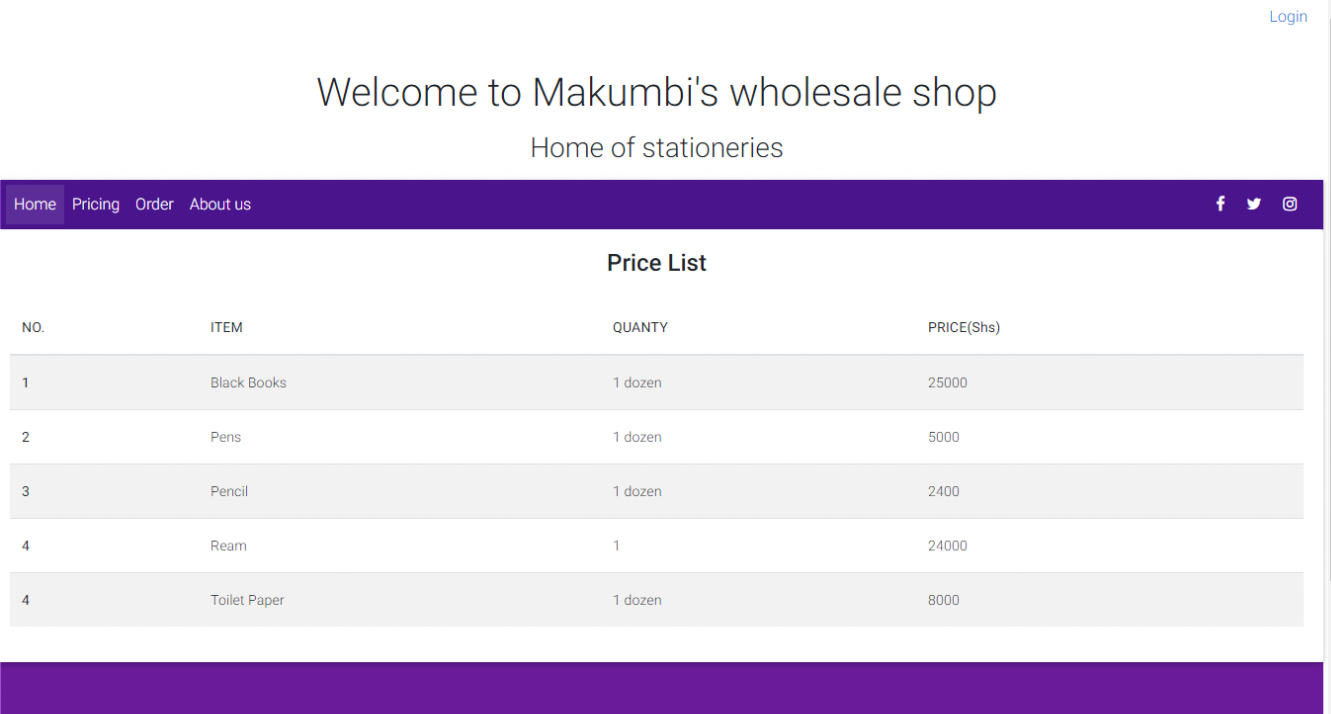
\includegraphics[width=\linewidth]{interface1.png}
\caption{ Shows the pricing interface}
\label{fig:Pricing}
\end{figure}
\begin{figure}
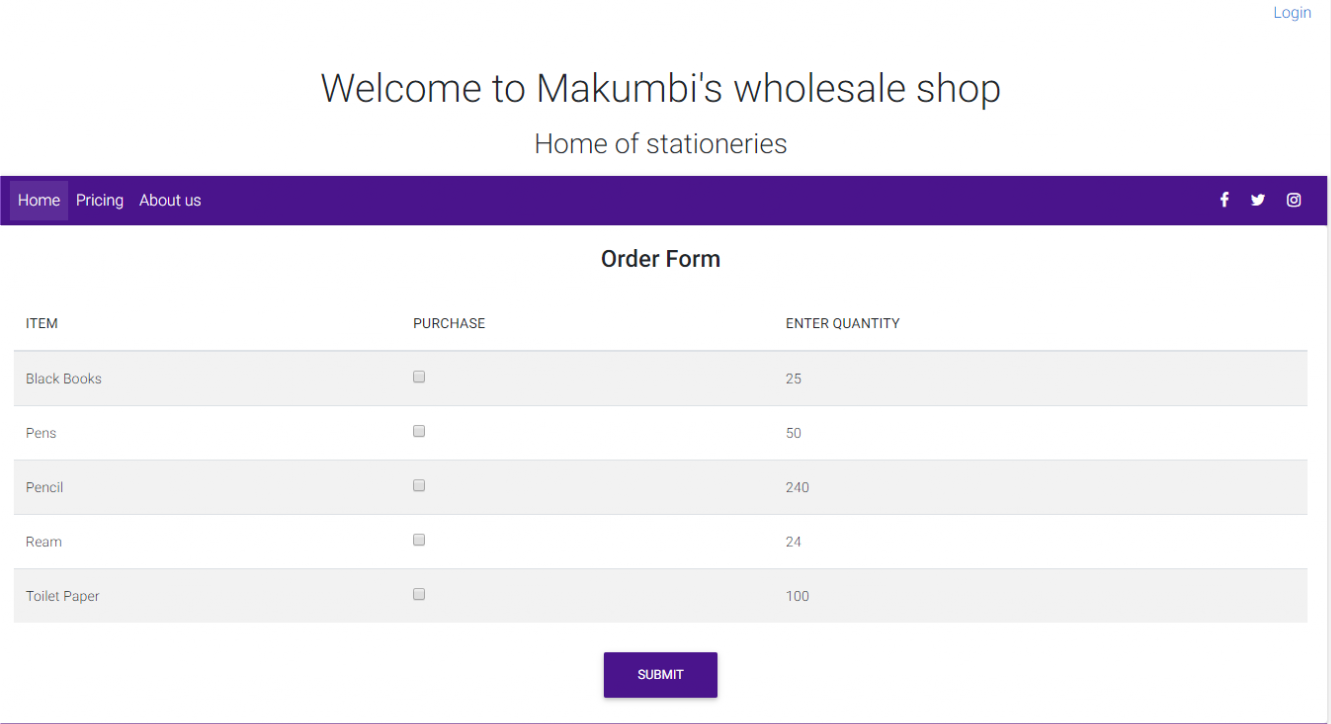
\includegraphics[width=\linewidth]{interface2.png}
\caption{ Shows the ordering interface}
\label{fig:Pricing}
\end{figure}
Figure \ref{fig:Pricing} shows the pricing interface
This final part of this study summarizes the research carried out, including the key finding and their implications. Thus, there are lots of recommendations which must be taken into considerations. These recommendation includes; changing the old manual system into a computerized system, organizing training workshops for employees to develop and improve their skills, and giving privilege to employee. Furthermore, other recommendations include the protection of the infrastructure needed for the new system (Hardware, Software, Users, Servers, Network protocol etc.), and ensuring periodic maintenance of the system, keeping backups of the data in case of unforseen circumstances.
\bibliographystyle{IEEEtran}
\bibliography{references}

\end{document}
